% 原PDF534–539／印刷503–508；全部原页已目视核对。
\clearpage\section*{常见分布表}\phantomsection\label{app:distributions}
\addcontentsline{toc}{section}{常见分布表}
\begingroup
\newcommand{\distheading}[1]{\par\medskip\needspace{10\baselineskip}\noindent\rule{\linewidth}{.3pt}\par\smallskip\noindent\textbf{#1}\par\smallskip}
\sourcepageanchor{534}
\subsection*{离散分布}
\distheading{伯努利分布（Bernoulli）$(p)$}
概率质量函数：$P(X=x\mid p)=p^x(1-p)^{1-x}$；$x=0,1$；$0\le p\le1$.
$$\text{均值与方差：}\quad EX=p,\qquad\operatorname{Var}X=p(1-p).$$
$$\text{矩母函数：}\quad M_X(t)=(1-p)+pe^t.$$

\distheading{二项分布（Binomial）$(n,p)$}
概率质量函数：$P(X=x\mid n,p)=\binom nx p^x(1-p)^{n-x}$；$x=0,1,2,\ldots,n$；$0\le p\le1$.
$$\text{均值与方差：}\quad EX=np,\qquad\operatorname{Var}X=np(1-p).$$
$$\text{矩母函数：}\quad M_X(t)=[pe^t+(1-p)]^n.$$
注：与二项式定理（\autoref{thm:3.2.2}）有关.多项分布（\autoref{def:4.6.2}）是二项分布的多元版本.

\distheading{离散均匀分布（Discrete Uniform）}
概率质量函数：$P(X=x\mid N)=\frac1N$；$x=1,2,\ldots,N$；$N=1,2,\ldots$.
$$\text{均值与方差：}\quad EX=\frac{N+1}{2},\qquad\operatorname{Var}X=\frac{(N+1)(N-1)}{12}.$$
$$\text{矩母函数：}\quad M_X(t)=\frac1N\sum_{i=1}^N e^{it}.$$

\distheading{几何分布（Geometric）$(p)$}
概率质量函数：$P(X=x\mid p)=p(1-p)^{x-1}$；$x=1,2,\ldots$；$0\le p\le1$.\footnote{译注：原表允许$p=0$，但在上述正整数支持上，此时总质量为0；作为通常的几何概率分布须有$0<p\le1$.下面的无记忆等式还需$s\ge t$为相应整数且条件事件概率为正.}
$$\text{均值与方差：}\quad EX=\frac1p,\qquad\operatorname{Var}X=\frac{1-p}{p^2}.$$
$$\text{矩母函数：}\quad M_X(t)=\frac{pe^t}{1-(1-p)e^t},\qquad t<-\log(1-p).$$
注：$Y=X-1$服从负二项$(1,p)$分布.该分布具有无记忆性：$P(X>s\mid X>t)=P(X>s-t)$.

\sourcepageanchor{535}
\distheading{超几何分布（Hypergeometric）}
\begin{equation*}\begin{aligned}
\text{概率质量函数：}\quad&P(X=x\mid N,M,K)=\frac{\binom Mx\binom{N-M}{K-x}}{\binom NK};\quad x=0,1,2,\ldots,K;\\
&M-(N-K)\le x\le M;\quad N,M,K\ge0.
\end{aligned}\end{equation*}
$$\text{均值与方差：}\quad EX=\frac{KM}{N},\qquad\operatorname{Var}X=\frac{KM}{N}\frac{(N-M)(N-K)}{N(N-1)}.$$
注：若$K\ll M$且$K\ll N$，则范围$x=0,1,2,\ldots,K$是适当的.\footnote{译注：原表只写$N,M,K\ge0$，通常还要求它们为整数、$M,K\le N$；所列方差公式在$N=1$等退化情形须另作解释.}

\distheading{负二项分布（Negative binomial）$(r,p)$}
概率质量函数：$P(X=x\mid r,p)=\binom{r+x-1}{x}p^r(1-p)^x$；$x=0,1,\ldots$；$0\le p\le1$.\footnote{译注：原表对$p$的端点约定有与几何分布相同的问题；通常取$r>0$、$0<p\le1$，按失败次数解释时$r$为正整数.}
$$\text{均值与方差：}\quad EX=\frac{r(1-p)}p,\qquad\operatorname{Var}X=\frac{r(1-p)}{p^2}.$$
$$\text{矩母函数：}\quad M_X(t)=\left(\frac{p}{1-(1-p)e^t}\right)^r,\qquad t<-\log(1-p).$$
注：概率质量函数的另一种形式为$P(Y=y\mid r,p)=\binom{y-1}{r-1}p^r(1-p)^{y-r}$，$y=r,r+1,\ldots$.该随机变量满足$Y=X+r$.负二项分布可以由泊松分布的伽马混合导出（见\autoref{exercise:4.32}\mbox{）.}

\distheading{泊松分布（Poisson）$(\lambda)$}
概率质量函数：$P(X=x\mid\lambda)=e^{-\lambda}\lambda^x/x!$；$x=0,1,\ldots$；$0\le\lambda<\infty$.
$$\text{均值与方差：}\quad EX=\lambda,\qquad\operatorname{Var}X=\lambda.$$
$$\text{矩母函数：}\quad M_X(t)=e^{\lambda(e^t-1)}.$$

\subsection*{连续分布}
\distheading{贝塔分布（Beta）$(\alpha,\beta)$}
概率密度函数：$f(x\mid\alpha,\beta)=\frac1{B(\alpha,\beta)}x^{\alpha-1}(1-x)^{\beta-1}$，$0\le x\le1$，$\alpha>0$，$\beta>0$.
$$\text{均值与方差：}\quad EX=\frac\alpha{\alpha+\beta},\qquad\operatorname{Var}X=\frac{\alpha\beta}{(\alpha+\beta)^2(\alpha+\beta+1)}.$$
$$\text{矩母函数：}\quad M_X(t)=1+\sum_{k=1}^{\infty}\left(\prod_{r=0}^{k-1}\frac{\alpha+r}{\alpha+\beta+r}\right)\frac{t^k}{k!}.$$
注：贝塔密度中的常数可以用伽马函数定义，$B(\alpha,\beta)=\frac{\Gamma(\alpha)\Gamma(\beta)}{\Gamma(\alpha+\beta)}$.式\eqref{eq:3.3.18}给出了矩的一般表达式.

\sourcepageanchor{536}
\distheading{柯西分布（Cauchy）$(\theta,\sigma)$}
$$f(x\mid\theta,\sigma)=\frac1{\pi\sigma}\frac1{1+((x-\theta)/\sigma)^2},\quad -\infty<x<\infty,\quad -\infty<\theta<\infty,\quad\sigma>0.$$
均值与方差：不存在.\qquad 矩母函数：不存在.

注：是自由度等于1的Student的$t$分布的特例.此外，若$X$与$Y$相互独立且均服从$n(0,1)$，则$X/Y$服从柯西分布.\footnote{译注：自由度为 $1$ 的通常 $t$ 分布和所写比值 $X/Y$ 对应的是标准柯西分布，即 $\theta=0,\sigma=1$. 表中一般的 $(\theta,\sigma)$ 分布须作位置尺度变换 $\theta+\sigma X/Y$.}

\distheading{卡方分布（Chi squared）}
$$f(x\mid p)=\frac1{\Gamma(p/2)2^{p/2}}x^{(p/2)-1}e^{-x/2};\quad0\le x<\infty;\quad p=1,2,\ldots.$$
$$\text{均值与方差：}\quad EX=p,\qquad\operatorname{Var}X=2p.$$
$$\text{矩母函数：}\quad M_X(t)=\left(\frac1{1-2t}\right)^{p/2},\qquad t<\frac12.$$
注：是伽马分布的特例.

\distheading{双指数分布（Double exponential）$(\mu,\sigma)$}
$$f(x\mid\mu,\sigma)=\frac1{2\sigma}e^{-|x-\mu|/\sigma},\quad-\infty<x<\infty,\quad-\infty<\mu<\infty,\quad\sigma>0.$$
$$\text{均值与方差：}\quad EX=\mu,\qquad\operatorname{Var}X=2\sigma^2.$$
$$\text{矩母函数：}\quad M_X(t)=\frac{e^{\mu t}}{1-(\sigma t)^2},\qquad |t|<\frac1\sigma.$$
注：也称为拉普拉斯分布（Laplace distribution）.

\distheading{指数分布（Exponential）$(\beta)$}
概率密度函数：$f(x\mid\beta)=\frac1\beta e^{-x/\beta}$，$0\le x<\infty$，$\beta>0$.
$$\text{均值与方差：}\quad EX=\beta,\qquad\operatorname{Var}X=\beta^2.$$
$$\text{矩母函数：}\quad M_X(t)=\frac1{1-\beta t},\qquad t<\frac1\beta.$$
注：是伽马分布的特例，具有无记忆性.有许多特殊变换：$Y=X^{1/\gamma}$服从威布尔分布，$Y=\sqrt{2X/\beta}$服从瑞利分布（Rayleigh），$Y=\alpha-\gamma\log(X/\beta)$服从耿贝尔分布\mbox{（Gumbel）.}

\sourcepageanchor{537}
\distheading{$F$分布}
\begin{equation*}\begin{aligned}
f(x\mid\nu_1,\nu_2)&=\frac{\Gamma((\nu_1+\nu_2)/2)}{\Gamma(\nu_1/2)\Gamma(\nu_2/2)}\left(\frac{\nu_1}{\nu_2}\right)^{\nu_1/2}\frac{x^{(\nu_1-2)/2}}{(1+(\nu_1/\nu_2)x)^{(\nu_1+\nu_2)/2}};\\
&\hspace{4em}0\le x<\infty;\qquad\nu_1,\nu_2=1,\ldots.
\end{aligned}\end{equation*}
均值与方差：
$$EX=\frac{\nu_2}{\nu_2-2},\quad\nu_2>2;\qquad\operatorname{Var}X=2\left(\frac{\nu_2}{\nu_2-2}\right)^2\frac{\nu_1+\nu_2-2}{\nu_1(\nu_2-4)},\quad\nu_2>4.$$
矩（矩母函数不存在）：
$$EX^n=\frac{\Gamma((\nu_1+2n)/2)\Gamma((\nu_2-2n)/2)}{\Gamma(\nu_1/2)\Gamma(\nu_2/2)}\left(\frac{\nu_2}{\nu_1}\right)^n,\qquad n<\frac{\nu_2}{2}.$$
注：与卡方分布有关（$F_{\nu_1,\nu_2}=(\chi_{\nu_1}^2/\nu_1)/(\chi_{\nu_2}^2/\nu_2)$，其中两个卡方变量相互独立），也与$t$分布有关（$F_{1,\nu}=t_\nu^2$）.

\distheading{伽马分布（Gamma）$(\alpha,\beta)$}
$$f(x\mid\alpha,\beta)=\frac1{\Gamma(\alpha)\beta^\alpha}x^{\alpha-1}e^{-x/\beta},\qquad0\le x<\infty,\quad\alpha,\beta>0.$$
$$\text{均值与方差：}\quad EX=\alpha\beta,\qquad\operatorname{Var}X=\alpha\beta^2.$$
$$\text{矩母函数：}\quad M_X(t)=\left(\frac1{1-\beta t}\right)^\alpha,\qquad t<\frac1\beta.$$
注：一些特例为指数分布（$\alpha=1$）与卡方分布（$\alpha=p/2,\beta=2$）.若$\alpha=3/2$，则$Y=\sqrt{X/\beta}$服从麦克斯韦分布（Maxwell）.$Y=1/X$服从逆伽马分布（inverted gamma distribution）.还可以与泊松分布联系起来（\autoref{ex:3.3.1}）.

\distheading{逻辑分布（Logistic）$(\mu,\beta)$}
$$f(x\mid\mu,\beta)=\frac1\beta\frac{e^{-(x-\mu)/\beta}}{[1+e^{-(x-\mu)/\beta}]^2},\quad-\infty<x<\infty,\quad-\infty<\mu<\infty,\quad\beta>0.$$
$$\text{均值与方差：}\quad EX=\mu,\qquad\operatorname{Var}X=\frac{\pi^2\beta^2}{3}.$$
$$\text{矩母函数：}\quad M_X(t)=e^{\mu t}\Gamma(1-\beta t)\Gamma(1+\beta t),\qquad |t|<\frac1\beta.$$
注：累积分布函数为$F(x\mid\mu,\beta)=\frac1{1+e^{-(x-\mu)/\beta}}$.

\distheading{对数正态分布（Lognormal）$(\mu,\sigma^2)$}
$$f(x\mid\mu,\sigma^2)=\frac1{\sqrt{2\pi}\sigma}\frac{e^{-(\log x-\mu)^2/(2\sigma^2)}}x,\quad0\le x<\infty,\quad-\infty<\mu<\infty,\quad\sigma>0.$$
$$\text{均值与方差：}\quad EX=e^{\mu+\sigma^2/2},\qquad\operatorname{Var}X=e^{2(\mu+\sigma^2)}-e^{2\mu+\sigma^2}.$$
$$\text{矩（矩母函数不存在）：}\quad EX^n=e^{n\mu+n^2\sigma^2/2}.$$
注：\autoref{ex:2.3.10}给出了具有相同各阶矩的另一个分布.

\sourcepageanchor{538}
\distheading{正态分布（Normal）$(\mu,\sigma^2)$}
$$f(x\mid\mu,\sigma^2)=\frac1{\sqrt{2\pi}\sigma}e^{-(x-\mu)^2/(2\sigma^2)},\quad-\infty<x<\infty,\quad-\infty<\mu<\infty,\quad\sigma>0.$$
$$\text{均值与方差：}\quad EX=\mu,\qquad\operatorname{Var}X=\sigma^2.$$
$$\text{矩母函数：}\quad M_X(t)=e^{\mu t+\sigma^2t^2/2}.$$
注：有时称为高斯分布（Gaussian distribution）.

\distheading{帕累托分布（Pareto）$(\alpha,\beta)$}
$$f(x\mid\alpha,\beta)=\frac{\beta\alpha^\beta}{x^{\beta+1}},\qquad\alpha<x<\infty,\quad\alpha>0,\quad\beta>0.$$
$$\text{均值与方差：}\quad EX=\frac{\beta\alpha}{\beta-1},\quad\beta>1;\qquad\operatorname{Var}X=\frac{\beta\alpha^2}{(\beta-1)^2(\beta-2)},\quad\beta>2.$$
矩母函数：不存在.

\distheading{$t$分布}
$$f(x\mid\nu)=\frac{\Gamma((\nu+1)/2)}{\Gamma(\nu/2)}\frac1{\sqrt{\nu\pi}}\frac1{(1+x^2/\nu)^{(\nu+1)/2}},\quad-\infty<x<\infty,\quad\nu=1,\ldots.$$
$$\text{均值与方差：}\quad EX=0,\quad\nu>1;\qquad\operatorname{Var}X=\frac\nu{\nu-2},\quad\nu>2.$$
矩（矩母函数不存在）：
\begin{equation*}\begin{aligned}
EX^n&=\frac{\Gamma((n+1)/2)\Gamma((\nu-n)/2)}{\sqrt\pi\Gamma(\nu/2)}\nu^{n/2},&&\text{若$n<\nu$且为偶数};\\
EX^n&=0,&&\text{若$n<\nu$且为奇数}.
\end{aligned}\end{equation*}
注：与$F$分布有关（$F_{1,\nu}=t_\nu^2$）.

\distheading{均匀分布（Uniform）$(a,b)$}
概率密度函数：$f(x\mid a,b)=\frac1{b-a}$，$a\le x\le b$.
$$\text{均值与方差：}\quad EX=\frac{b+a}{2},\qquad\operatorname{Var}X=\frac{(b-a)^2}{12}.$$
$$\text{矩母函数：}\quad M_X(t)=\frac{e^{bt}-e^{at}}{(b-a)t}.$$
注：若$a=0$且$b=1$，这是贝塔分布（$\alpha=\beta=1$）的特例.\footnote{译注：此处密度需$a<b$；矩母函数在$t=0$处按连续延拓取1.原表未显写这两项约定.}

\sourcepageanchor{539}
\distheading{威布尔分布（Weibull）$(\gamma,\beta)$}
$$f(x\mid\gamma,\beta)=\frac\gamma\beta x^{\gamma-1}e^{-x^\gamma/\beta},\qquad0\le x<\infty,\quad\gamma>0,\quad\beta>0.$$
均值与方差：
$$EX=\beta^{1/\gamma}\Gamma\!\left(1+\frac1\gamma\right),\qquad\operatorname{Var}X=\beta^{2/\gamma}\left[\Gamma\!\left(1+\frac2\gamma\right)-\Gamma^2\!\left(1+\frac1\gamma\right)\right].$$
矩：\footnote{译注：原页的矩公式漏印了伽马函数符号；对非负整数$n$应为$EX^n=\beta^{n/\gamma}\Gamma(1+n/\gamma)$，这也与上方的一阶矩公式一致.}
$$EX^n=\beta^{n/\gamma}\left(1+\frac n\gamma\right).$$

注：矩母函数仅在$\gamma\ge1$时存在，其形式并不十分有用.一个特例是指数分布\mbox{（$\gamma=1$）.}

\clearpage
\begin{center}
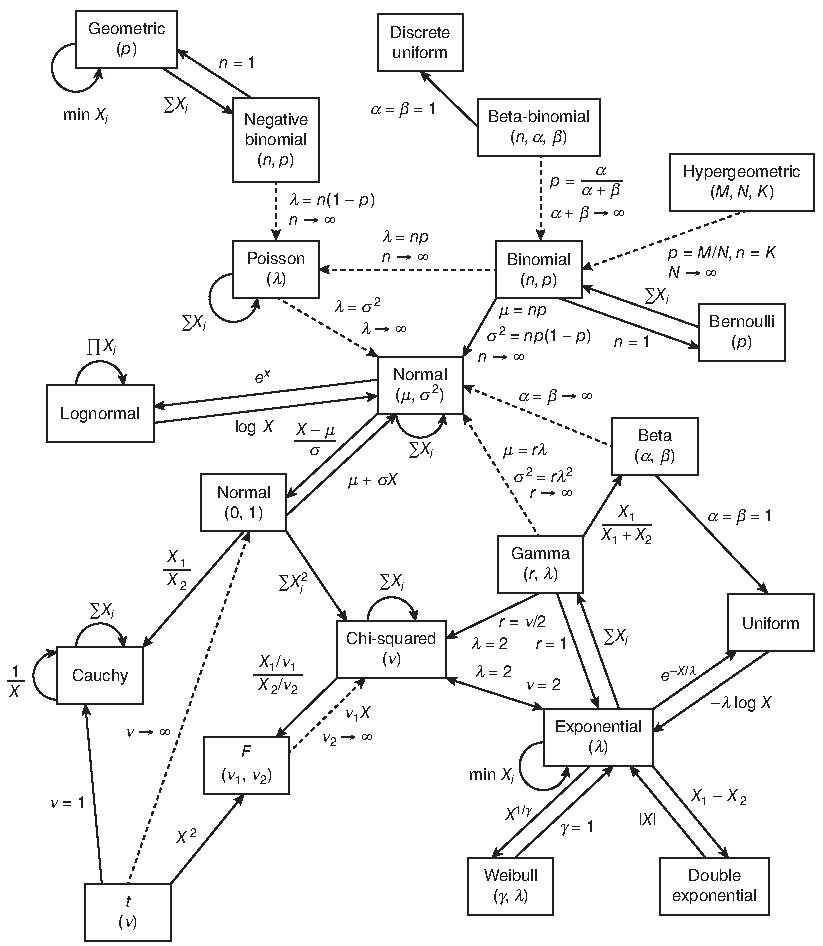
\includegraphics[width=.94\textwidth,height=.80\textheight,keepaspectratio]{assets/backmatter/distribution-relations.pdf}
\end{center}
\noindent\textbf{常见分布之间的关系.}实线表示变换与特例，虚线表示极限.据\hyperref[bib:source195]{Leemis（1986）}改编.

\smallskip\noindent\small 图中名称中英对照：Geometric—几何；Discrete uniform—离散均匀；Negative binomial—负二项；Beta-binomial—贝塔二项；Hypergeometric—超几何；Poisson—泊松；Binomial—二项；Bernoulli—伯努利；Lognormal—对数正态；Normal—正态；Beta—贝塔；Gamma—伽马；Chi-squared—卡方；Uniform—均匀；Cauchy—柯西；Exponential—指数；Weibull—威布尔；Double exponential—双指数.
\endgroup
